\documentclass[11pt]{article}

\usepackage[margin=1.5in]{geometry}
\usepackage{amsmath,amssymb,amsthm}
\usepackage{enumitem}
\usepackage{hyperref}
\usepackage{mathtools}
\usepackage{tikz}
\usetikzlibrary{arrows.meta,positioning,calc}

\theoremstyle{definition}
\newtheorem{definition}{Definition}
\newtheorem{example}{Example}
\newtheorem{remark}{Remark}
\newtheorem{theorem}{Theorem}
\newtheorem{proposition}{Proposition}
\usepackage{float}
\usepackage[normalem]{ulem}

\title{Lecture 1: Vectors, Matrices, and Linear Systems}
\author{Handout Notes}
\date{}

\begin{document}

\maketitle

\section*{Overview}
This first lecture comprises three sessions.

\begin{itemize}
    \item Session 1: Introduction to the course, Linear Systems and three pictures of systems 
    \item Session 2: Elimination and elementary row operations
    \item Session 3: Existence and Uniqueness of solutions, Row Echelon Forms, and Gauss-Jordan Elimination
\end{itemize}

\section{Fundamentals of Linear Algebra}

The ultimate goal of linear algebra is to \textbf{solve a system of linear equations}

\begin{itemize}
    \item \textbf{Equation:} a mathematical statement that asserts the equality of two expressions
    \item \textbf{System:} a collection of one or more equations involving the same set of variables
    \item \textbf{Solution:} find all values of the unknowns that satisfy every equation in the system
\end{itemize}

\textbf{Linear Equation:} A linear equation in the variables $x_1, x_2, \ldots, x_n$ is an equation that can be written in the form
\[
    a_1x_1 + a_2x_2 + \cdots + a_nx_n = b,
\]
where $b$ and the coefficients $a_1, a_2, \ldots, a_n$ are real numbers.

\textbf{Character of linear equations:} \sout{each term is either a constant or the product of a constant and a single variable (first power).} Maximum power of unknown is 1.
\begin{itemize}
    \item $a_1x_1 + a_2x_2$ is linear
    \item $a_1x_1 + x_1x_2$ is not linear
\end{itemize}

Linear combinations preserve two properties: \textbf{additivity} and \textbf{homogeneity}.

\begin{itemize}
    \item Additivity preserves addition, i.e., $f(x+y) = f(x) + f(y)$
    \item Homogeneity preserves scalar multiplication, i.e., $f(cx) = cf(x)$
\end{itemize}



\subsection{Representation of Linear System}

\begin{figure}[H]
\centering
\fbox{
\begin{tikzpicture}[>=Latex, every node/.style={font=\small}]
    % left side variables
    \node[draw, minimum width=1.2cm, minimum height=1.2cm] (x) at (0,1.5) {$x$};
    \node[draw, minimum width=1.2cm, minimum height=1.2cm] (y) at (0,-1.5) {$y$};

    % arrows from x and y to the right
    \draw[->] (x.east) -- ++(1.5,0) node[midway, above] {1};
    \draw[->] (y.east) -- ++(1.5,0) node[midway, above] {2};

    % output block
    \node[draw, minimum width=2.2cm, minimum height=4.3cm, align=center] (R) at (5,0) {Output};

    % arrows entering the right block
    \draw[->] ($(R.west)+(-1.2,1.2)$) -- ++(1.2,0) node[midway, above] {1};
    \draw[->] ($(R.west)+(-1.2,-1.2)$) -- ++(1.2,0) node[midway, above] {4};
\end{tikzpicture}
}
\caption{Basic Battery Manufacturing: Module X (Ore Machine) produces 1 unit of ore. Module Y (Gel Machine) produces 2 units of energy gel. Final input takes 1 ore and 4 gel to produce Battery Lv. I.}
\label{fig:linear_system_schematic}

\end{figure}

As shown in \autoref{fig:linear_system_schematic}, to find the solution of how many X and Y, we can solve either the equation of:

\[
\begin{cases}
    1x + 0y= 1,\\
    0x + 2y = 4,
\end{cases}
\]

whose solution is \((x,y)=(1,2)\).



\subsection{Three Pictures of Linear System}


Consider the linear system
\[
\begin{cases}
2x-y=0,\\
-x+2y=3.
\end{cases}
\]
This is a system of two equations in two unknowns. 

\paragraph{Row Picture} In row picture, we depict the function image and find if there is an intersection point. 

\begin{figure}[H]
\centering
\fbox{
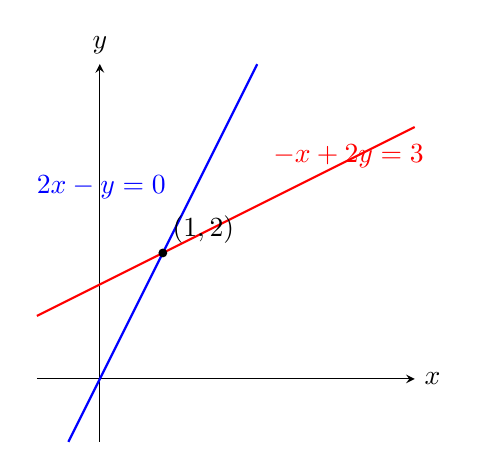
\begin{tikzpicture}[scale=0.8,>=stealth]
  \draw[->] (-1,0) -- (5,0) node[right] {$x$};
  \draw[->] (0,-1) -- (0,5) node[above] {$y$};

  % line 2x - y = 0  =>  y = 2x
  \draw[blue,thick,domain=-0.5:2.5,samples=100] plot (\x,{2*\x});
  % line -x + 2y = 3 => y = (x+3)/2
  \draw[red,thick,domain=-1:5,samples=100] plot (\x,{(\x+3)/2});

  % intersection point
  \fill (1,2) circle (2pt);
  \node[above right] at (1,2) {$(1,2)$};

  \node[above left,blue] at (1.2,2.7) {$2x-y=0$};
  \node[above right,red] at (2.6,3.2) {$-x+2y=3$};
\end{tikzpicture}
}
\caption{Row picture of the system \(2x-y=0\) and \(-x+2y=3\).}
\end{figure}

\paragraph{Column Picture} In column picture, we depict the vectors and combine them. After that, move around until we see the combined vector points to the (0,3). The solution is the origin of the final vector.

\begin{figure}[H]
\centering
\fbox{
\begin{tikzpicture}[scale=0.8,>=stealth]
      \draw[->] (-2,0) -- (3,0) node[right] {$x$};
      \draw[->] (0,-3) -- (0,4) node[above] {$y$};

      % translated vectors
      \draw[black, thick, ->] (0,0) -- (2,-1) node[below right] {$1\begin{bmatrix}2\\-1\end{bmatrix}$};
      \draw[black, thick, ->] (0,0) -- (-2,4) node[above left] {$2\begin{bmatrix}-1\\2\end{bmatrix}$};
      \draw[black, thick, ->] (0,0) -- (-1,2) node[above left] {};

      % vector b
      \draw[red, thick, ->] (0,0) -- (0,3) node[above right, text=red] {$\mathbf{b}$};
      \fill[red] (0,0) circle (2pt);
    %   \node[below left, red] at (-2,-1) {start $=(0,0)$};
      \node[above right, red] at (1,3) {$(0,3)$};

      \draw[dotted, black, thick] (2,-1) -- (0,3);
      \draw[dotted, black, thick] (-2,4) -- (0,3);
\end{tikzpicture}
}
\caption{Column picture of the system showing the vector combination $1\begin{bmatrix}2\\-1\end{bmatrix} + 2\begin{bmatrix}-1\\2\end{bmatrix} = \begin{bmatrix}0\\3\end{bmatrix}$.}
\end{figure}

\paragraph{Matrix}  In matrix form, it is
\[
\begin{pmatrix}
2 & -1 \\
-1 & 2
\end{pmatrix}
\begin{pmatrix}x\\y\end{pmatrix}
=
\begin{pmatrix}0\\3\end{pmatrix}.
\]

Or, we can write it as:
\[
\left[
\begin{array}{cc|c}
2 & -1 & 0 \\
-1 & 2 & 3
\end{array}
\right].
\]

That is the \textbf{augmented matrix}.

\subsection{Properties of Linear Equation Systems}


\paragraph{Dimension of System} Linear systems may have n variables (columns) and m equations (rows). We name them m $\times$ n (linear) system.

Ideally, we like the ones where m = n, because it is \textit{likely} to have a unique solution. 

\vspace{0.5em}
\noindent\fbox{%
    \begin{minipage}{\textwidth}
        Think: why it is likely to have a unique solution?\\
        {\color{white} While m = n, some equations may be merged if they are equivalent. If so, m $<$ n, and solution won't be unique.}
    \end{minipage}%
}

\paragraph{Consistency of System} A linear system is \textbf{consistent} if it has at least one solution. Otherwise, it is \textbf{inconsistent}.


\paragraph{Equivalent Systems} Two linear systems are \textbf{equivalent} if they have the same solution set.


\vspace{0.5em}
\noindent\fbox{%
    \begin{minipage}{\textwidth}
        Think: what characterizes a linear system? What is the difference between consistency and equivalence?\\
        {\color{white} Solution sets. Consistency is for equations. Equivalence is for systems.}
    \end{minipage}%
}

\subsection{Solution Sets}
How many solutions can a linear system have?

\begin{itemize}
    \item 1, when the lines intersect at a single point
    \item 0, for example, when the lines are parallel
    \item $\inf$, when lines overlap
\end{itemize}



\vspace{0.5em}
\noindent\fbox{%
    \begin{minipage}{\textwidth}
        Think: is it possible for linear system to have 2 solutions?\\
        {\color{white} :( You are free to think why it is impossible.}
    \end{minipage}%
}
\section{Elimination}
A system is characterized by its solution set. To solve a system, we perform elimination.

\begin{itemize}
    \item \textbf{Input:} a system of linear equations.
    \item \textbf{Output:} an "Echelon form" system
    \item \textbf{Actions:} elementary row operations
\end{itemize}

\subsection{Elementary Row Operations}
There are three elementary operations that produces equivalent systems:

\begin{itemize}
    \item Interchange: swap rows. Equations are not ordered
    \item Scaling: multiply a row by a (non-zero) constant. Linear systems preserve multiplication.
    \item Replacement: add a multiple of one row to another row. Linear systems preserve addition.
\end{itemize}


\vspace{0.5em}
\noindent\fbox{%
    \begin{minipage}{\textwidth}
        Think: how do we ensure the elimination to be feasible?
        {\color{white} Row operations produces equivalent systems.}
    \end{minipage}%
}

\subsection{Coefficient Matrix}
Recall that we discussed the three pictures of linear systems. Coefficient matrix is a compact representation of the system. Only the coefficients of variables are stored. The coefficient of the $m^th$ equation's $n^{th}$ variable is stored in the $m^{th}$ row and $n^{th}$ column of the matrix.

For the $3\times 3$ linear system
\[
\begin{cases}
    x + 2y - z = 1,\\
    2x - y + 3z = 7,\\
    -x + 4y + 2z = 5.
\end{cases}
\]

Its coefficient matrix is

\[
\begin{bmatrix}
    1 & 2 & -1\\
    2 & -1 & 3\\
    -1 & 4 & 2
\end{bmatrix}.
\]

\subsection{Augmented Matrix}
We do need the numbers to the right of equal sign. When we add them to the right, we create a \textbf{augmented matrix}. 
\[
\left[
\begin{array}{ccc|c}
    1 & 2 & -1 & 1\\
    2 & -1 & 3 & 7\\
    -1 & 4 & 2 & 5
\end{array}
\right].
\]

\subsection{Echelon Form}
When performing elimination, we want to only keep $x_1$ on the 1st row (rest rows do not have $x_1$), only keep $x_2$ on the 2nd row (rest rows do not have $x_2$), and so on. For the system above, after elimination, we get:

\[
\left[
\begin{array}{ccc|c}
    1 & 2 & -1 & 1 \\
    0 & -2.5 & 2.5 & 2.5 \\
    0 & 0 & 7 & 12
\end{array}
\right],
\]

we have zeros below the leading entries in each column. Consequently, this is called \textbf{Echelon Form}.

\subsection{Pivot Elements}
\begin{itemize}
    \item Nonzero row or column: a row or column that contains at least one nonzero entry.
    \item Pivot column: leftmost nonzero column
    \item Pivot: nonzero entry at the top of pivot column
    \item Pivot row: row that contains a pivot
\end{itemize}

Basically speaking, because there can be many zeros in a row or column, we only care about, after the matrix has been sorted out, the first entry and corresponding entries afterwards.


\subsection{Elementary Row Reduction}
\begin{itemize}
    \item Begin with leftmost nonzero column. This is a pivot column. The pivot position is at the top.
    \item Select the pivot (nonzero entry at the begining). Let's start from the first unknown corresponding to $x_1$, for example.
    \item Perform elementary row operation for all other entris in the column. As such, we eliminate all $x_1$ \textbf{except} for the selected row.
    \item Continue with column \#2, \#3, and so on.
\end{itemize}


\vspace{0.5em}
\noindent\fbox{%
    \begin{minipage}{\textwidth}
        Think: is echelon form unique?\\
        {\color{white} No. There are many ways to perform elimination.}
    \end{minipage}%
}


\subsection{How to Tell An Echelon Form}
Well, as you may realize, not all systems are "beautiful". There are "talllllll" systems (Much more equations than unknowns), and "wiiiiiiiiide" systems (Much more unknowns than equations).

Whatever it may be, remember that the basic idea of echelon form is to allow us tell what is the solution immediately. 

Ideally, you can see a perfect "stair": if we forget zeros in the matrix, the first row starts from column 1, second row starts from column 2, \dots

If the system is "tallllll" (M $>$ N), then the last rows are all zeros, because the maximum non-zero rows is the number of unknowns.

If the system is wiiiiide (N $>$ M), then there are columns not having leading entries. 

\paragraph{For example:}
\[
\left[
\begin{array}{cccc|c}
    1 & 0 & 2 & 1 & 4 \\
    0 & 0 & -1 & 2 & 3 \\
    0 & 0 & 0 & 3 & 1
\end{array}
\right]
\]

Here, the second variable $x_2$ is all 0. This is a \textbf{free variable}, while $x_1$, $x_3$, and $x_4$ are corresponding to a pivot (1, -1, and 3, separately). They are the \textbf{basic variables}. 

It is fine to have free variables, but make sure to order the rows that the appearance of other non-zero pivots are $\searrow$.

\vspace{0.5em}
\noindent\fbox{%
    \begin{minipage}{\textwidth}
        Think: when may a consistent system have infinitely many solutions?\\
        {\color{white} Containing free variables}
    \end{minipage}%
}


\section{Existence, Uniqueness, and Gaussian Elimination}
\subsection{Fundamental Questions in Linear System}
We said that the most important thing we care about in linear algebra is to solve the system towards solution sets.

But it is more important to know beforehand whether the system even has a solution:

1) Is the system consistent, so that a solution exist?

2) If a solution exists, is it unique?

\paragraph{Key Observations.} 

\begin{itemize}
    \item All zero row $\Rightarrow$ inconsistent system.
    \[
\left[
\begin{array}{ccc|c}
0 & 0 & 0 &b
\end{array}
\right].
\]
    \item Free variable $\Rightarrow$ infinitely many solutions.
    \item One unique solution $\Leftarrow$ $num(var_{lead}) = num(var_{total})$.
\end{itemize}

\subsection{Gaussian Elimination}
In math, we care about a solution, but also care about "the" solution that is unique, minimal, or simplest.

Row echelon form is not unique. That is the issue. For you folks, if I ask you to reduce to row echelon form, my TA and I will get mad --- if I really did ask you to do a row echelon form, you can torture me with millions of ways.

\[\left[
\begin{array}{cccc|c}
    100&0  & 200 & 100 & 400 \\
    0 & 0 & -1.414 & 2.828 & 4.242 \\
    0 & 0 & 0 & 81930 & 27310
\end{array}
\right]
\]

This $\uparrow$ is a row echelon form!!!!

To make our lives easier, we have Gauss-Jordan Elimination to minify this echelon form. And it is super easy, because it is exactly how you write the solution like 

\[
\begin{cases}
x \quad \quad= 9,\\
\quad y + \quad= 1,\\
\quad \quad z = 6
\end{cases}
\]

It creates a fancy matrix

\[
\left[
\begin{array}{ccc|c}
    1 & 0 & 0& 9 \\
    0 & 1 & 0 & 1 \\
    0 & 0 & 1 & 6
\end{array}
\right]
\]

\subsection{Reduced Row Echelon Form}
A reduced row echelon form satisfies:
\begin{itemize}
    \item It is in row echelon form.
    \item The first nonzero (leading) entry in each nonzero row is 1.
    \item Each leading 1 is the \textbf{only} nonzero entry in its \textbf{column}. (For each pivot, above and below are all zeros)
\end{itemize}

\paragraph{How to get reduced row echelon form}

\begin{itemize}
    \item Step 1: reduce to row echelon form
    \item Step 2: scale each pivot row to make the leading entry 1
    \item Step 3: eliminate each column creating zeros above and leftwards
\end{itemize}

\vspace{0.5em}
\noindent\fbox{%
    \begin{minipage}{\textwidth}
        Think: when could reduced echelon form ever have a column containing numbers that is neither 0 nor 1?\\
        {\color{white} When there is a free variable or it is inconsistent.}
    \end{minipage}%
}

\subsection{Let's Formalize "TALL" and "WIDE"}
Recall that we mentioned "Talllll" and "Wiiiide" systems.

\paragraph{Overdetermined}: the number of equations is more than the number of unknowns. It is a "Tall" system. 

\paragraph{Underdetermined}: the number of equations is less than the number of unknowns. It is a "Wide" system.

\vspace{0.5em}
\noindent\fbox{%
    \begin{minipage}{\textwidth}
        Think: must an overdetermined system be inconsistent? \\
        Must an underdetermined system have infinitely many solutions? \\
        Is it possible for underdetermined system to have a unique solution?\\
        {\color{white} Not necessarily.\\If consistent, yes\\Not possible}
    \end{minipage}%
}

\subsection{Rank of a Matrix}

The rank of a matrix $A$, denoted $\text{r}(A)$, is the  number of nonzero rows in reduced row echelon form. For m $\times$ n matrix, we have $\text{r}(A) \leq \min(m,n)$.

Rank of a matrix is important to determine the existence and uniqueness of solution. For example, given a linera system (I know, this is an inconsistent system):

\[
\begin{cases}
x+3z=1,\\
y+2z=0,\\
0=1
\end{cases}
\]

We have the Coefficient Matrix $A$ to be 
\[
\bar{A}=
\left[
\begin{array}{ccc}
1 & 0 & 3 \\
0 & 1 & 2 \\
0 & 0 & 0 
\end{array}
\right]
\]

... and Augmented Matrix $\bar{A}$ to be
 Given an original augmented matrix $\bar{A}$:

\[
\bar{A}=
\left[
\begin{array}{ccc|c}
1 & 0 & 3 & 1\\
0 & 1 & 2 & 0\\
0 & 0 & 0 & 1
\end{array}
\right]
\]

Refer to ppt slide no. 81, we know that this is an echelon form because 1) the number of leading 0 of nonzero rows strictly increases (see the downright diagonal shape of zeros to the bottom left?) and 2) all zero rows (if any) are at the bottom, which we do not have.

Refer to ppt slide no. 98, We also know that this is a reduced echelon form because 1) it is an echelon form, 2) the first nonzero entry for each nonzero row is 1, and 3) first nonzero entry in each row is the only nonzero entry in its column.

Also, unfortunately, this is inconsistent, because we observe an ugly row at the bottom with all 0s on the left and a non-zero number on the right. If the non-zero number is 0, then it is consistent. Unfortunately, it is not.


We can also use rank to determine. 

First, linear system is \textbf{consistent} only when it has no form of [ 0 \dots 0 b ], so it is not consistent. In another word, matrix is consistent only if \textbf{the rank of augmented matrix} $\bar{A}$ equals \textbf{the rank of coefficient matrix} $A$.

Second, if a linear system is consistent, the amount of solution depends on \textbf{whether there is a free variable}. The number of free variable is determined by the difference between the rank of the coefficient matrix $A$ (rank is 2 because there is an all-0 row) and the augmented matrix $\bar{A}$ (rank is 3 because there is a 1 in the third row of augmented matrix).

If we say $r= r(\bar{A}) $ and $ n = r(A) $, as $\bar{A}$ is a reduced form, it is always $r \leq n$, and there are $n - r$ free variables.

When summed together:
\begin{itemize}
    \item If $r = n$, this is the only case to tell A is consistent.
    \item If $r < n$: this depends. If consistent, then there are infinitely many solutions, with $n-r$ free variables
\end{itemize}


In this case, $r$ = 2 and $n$=3, so even it is consistent, there is one free variable and we have infinitely many solutions.

Beautiful, isn't it?

\section{Summary}

\begin{enumerate}
    \item This lecture, we cover the basic ideas of linear systems. We start from the fundamental question of how to solve linear systems (by the way, do you remember what is linear?). 
    \item To solve a system, we have three pictures to refer to. The row picture is drawing lines of functions. The column picture is to draw vectors. And the matrix.
    \item We learn that there are three cases of solutions: one unique, infinitely many, zero. To understand why there can be zero solutions, we introduce the idea of consistency.
    \item We learn how to perform elimination on coefficient matrix by reducing it to echelon form. We introduce concepts around pivot.
    \item We learned elementary row operation to perform reduction. Nothing too hard, just what we applied with equation systems.
    \item We realize that row echelon form has a problem of not being unique, and we explore a way to perform unique result by Gaussian Elimination. The basic idea is to fix each variable's coefficient to 1 and eliminate all possible entries.
    \item We discussed possible conditions of row reduced echelon form by applying the Gaussian algorithm, and revisited the consistency of matrices.
    \item To further understand the solution sets to systems and why we love systems with N equations and N variables, we learn the rank of a matrix, and learn how to use it to determine the existence and uniqueness of solutions. 

\end{enumerate}


As such, this lecture is centered around solutions to linear systems, the existence and uniqueness. We use elementary row operations to manipulate matrix retaining its equivalence. We determine the existence and uniqueness by assessing the consistency. And we learn how to reduce the matrix to the utmost simple form to solve them.

\section{In the Next Episode...}
We will look at the linear algebra in "column view". We will learn how vectors can be represented, operated, and solved with matrices. We will particularly solve the tricky "multiplication" of vectors, and learn how can an object be transformed in the space under matrix representation. 

But before that, good luck with the assignments :3
\end{document}
